\section{Performance Tuning}
\label{section:performance}

\subsection{NAMD performance tuning concepts}
The simulation performance obtained from NAMD depends on many factors.
The particular simulation protocol being run is one of the largest
single factors associated with NAMD performance, as different simulation
methods invoke different code that can have substantially different 
performance costs, potentially with a different degree of parallel
scalability, message passing activity, hardware acceleration through
the use of GPUs or CPU vectorization,
and other attributes that also contribute to overall NAMD performance.

\paragraph{Measuring performance.}
When NAMD first starts running, it does significant I/O, FFT tuning,
GPU context setup, and other work that is unrelated to normal 
simulation activity, so it is important to measure performance only
when NAMD has completed startup and all of the processing units are
running at full speed.
The best way to measure NAMD performance accurately requires running
NAMD for at least 500 to 1,000 steps of normal dynamics (not minimization),
so that load balancing has a chance to 
take place several times, and all of the CPUs and GPUs have ramped up
to 100\% clock rate.  NAMD provides ``Benchmark time:'' and ``TIMING:''
measurements in its output, which can be used for this purpose.  
Here, we are only interested in the so-called wall clock time.

Modern GPU performance is now so fast,
especially for GPU-resident mode,
that it is expected to take a much longer run than 1,000 steps
for hardware to achieve a steady thermal state and power utilization
reflecting true long-term simulation performance behavior.
The following config parameter can be used to run
dynamics for some number of seconds.
\begin{itemize}
\item
\NAMDCONF{benchmarkTime}
{Perform benchmark for indicated number of seconds}
{positive integer}{%
Use for benchmarking dynamics. Terminate simulation after running for
the indicated number of seconds, where the termination condition is
checked at the next ``TIMING:'' output.
}
\end{itemize}
A reasonable benchmark length might be in the range of 120 to 180
(two to three minutes) to provide enough time
for the hardware to fully warm up.
If \texttt{outputPerformance} is left enabled (the default setting)
the final ``PERFORMANCE:'' line will show
the average ns/day performance.
A good value for \texttt{outputTiming} might be 100, 500,
or even 1000, depending on the system size and hardware capability,
where performance monitoring should probably not be done more than
once per second of wall time.
These practices are now the preferred way to benchmark GPU-accelerated
builds of NAMD, because the measurements shown by the
``Benchmark time:'' output lines are gathered too quickly
in the simulation to accurately determine true performance.


\paragraph{NAMD configuration and I/O performance.}
Aside from the choice of major simulation protocol and associated
methods in use, it is also important to consider the performance impacts
associated with routine NAMD configuration parameters such as those
that control the frequency of simulation informational outputs and 
various types of I/O.
Simulation outputs such as energy information may require NAMD to do additional
computations above and beyond standard force evaluation calculations.
We advise that NAMD simulation configuration parameters be selected such
that output of energies (via the \texttt{outputEnergies} parameter) 
be performed only as much as is strictly necessary, since 
they otherwise serve to slow down the simulation due to the extra
calculations they require.  
NAMD writes ``restart" files to enable simulations that were terminated 
unexpectedly (for any reason) to be conveniently restarted from the 
most recently written restart file available.  While it is desirable
to have a relatively recent restart point to continue from, writing
restart information costs NAMD extra network communication and disk I/O.
If restart files are written too frequently, this extra activity and I/O
will slow down the simulation.  A reasonable estimate for restart
frequency is to choose the value such that NAMD writes restart files
about once every ten minutes of wall clock time.  
At such a rate, the extra work and I/O associated with writing
the restart files should remain an insignificant factor in NAMD performance.

\paragraph{Computational (arithmetic) performance.}
NAMD is provided in a variety of builds that support platform-specific
techniques such as CPU vectorization and GPU acceleration 
to achieve higher arithmetic performance, thereby increasing 
NAMD simulation throughput.  
Whenever possible NAMD builds should be compiled such that 
CPU vector instructions are enabled, and highly tuned
platform-specific NAMD code is employed for performance-critical 
force computations.
The so-called ``SMP'' builds of NAMD benefit from reduced memory use 
and can in many cases perform better overall, but one trade-off 
is that the communication thread is unavailable for simulation work.
NAMD performance can be improved by explicitly setting CPU affinity
using the appropriate Charm++ command line flags, e.g., 
\texttt{++ppn 7 +commap 0,8 +pemap 1-7,9-15} as an example.

It is often beneficial to reserve one CPU core for the 
operating system, to prevent harmful operating system noise or ``jitter'',
particularly when running NAMD on large scale clusters or supercomputers.
The Cray \texttt{aprun -r 1} command reserves and
forces the operating system to run on the last CPU core.

State-of-the-art compute-optimized GPU accelerators, 
can provide NAMD with simulation performance equivalent to 
several CPU sockets (on the order of 100 CPU cores) when used to 
greatest effect, e.g., when GPUs have sufficient work per GPU.
In general, effective GPU acceleration currently requires on the order
of 10,000 to 100,000 atoms per GPU assuming a fast network interconnect.
NAMD GPU-offload mode requires several CPU cores to drive each GPU effectively,
ensuring that there is always work ready and available for the GPU.
For contemporary CPU and GPU hardware, the most productive ratios of 
CPU core counts per GPU might range from 8:1 to 64:1 or higher depending on
the details of the hardware involved.
GPU-offload mode running on modern GPU hardware will be
bottlenecked by the CPU, which means that it is especially important
to follow NUMA domain mapping considerations and generally avoid
running other than one hardware thread per core
(i.e., SMT 1, avoiding use of ``hyper-threading'').
An advantageous hardware configuration might have one NUMA domain
per GPU, which is used most effectively by scheduling one
SMP rank per GPU device / NUMA domain, again leaving at least
one core per NUMA domain available for the communication thread.

GPU-resident mode shifts almost all computational work to the GPU
so generally requires less CPU core support per device than GPU-offload mode,
where the CPU is used primarily for GPU kernel management
and doing infrequent bursts of activity related to atom migration and file I/O
or possibly doing frequent bursts of activity if some host-based
computation such as Colvars is used.
GPU-resident mode uses shared-memory parallelism
but is capable of scaling across multiple GPUs on the same physical node
when the GPUs are interconnected by a high-speed networking fabric,
such as NVLink or NVSwitch for NVIDIA or Infinity Fabric for AMD.
For standard simulations, CPU involvement is low enough
to be unaffected by NUMA domain issues.
However, heavier per-step use of the CPU cores,
such as using Colvars with GPU-resident mode,
might benefit from mapping device PEs to a shared NUMA domain.


\paragraph{Networking performance.}
When running NAMD on more than a single node, it is important to 
use a NAMD version that is optimal for the underlying network hardware
and software you intend to run on.  The Charm++ runtime system on which
NAMD is based supports a variety of underlying networks, so be sure to
select a NAMD/Charm++ build that is most directly suited for your 
hardware platform.  In general, we advise users to avoid the use of 
an MPI-based NAMD build as it will underperform compared with a native
network layer such as InfiniBand IB verbs (often referred to as ``verbs''),
the UCX (Unified Communication X) framework (``ucx''),
%the Cray-specific ``gni-crayxc'' or ``gni-crayxe'' layer,
the Cray-specific ``ofi-crayshasta'' (or ``ofi-crayshasta cxi'') layer
for Slingshot-11,
or the IBM PAMI message passing layer, as practical examples.


\subsection{Non-bonded interaction distance-testing}

The last critical parameter for non-bonded
interaction calculations is the parameter {\tt pairlistdist}.  To reduce the
cost of performing the non-bonded interactions, \NAMD\ uses a {\it non-bonded
pair list} which contained all pairs of atoms for which
non-bonded interactions
should be calculated.  Performing the search for pairs of atoms that
should have their interactions calculated is an expensive operation.  Thus,
the pair list is only calculated periodically, at least once per cycle.
Unfortunately,
pairs of atoms move relative to each other during the steps between preparation
of the pair list.  Because of this, if the pair list were built to include
only
those pairs of atoms that are within the cutoff distance
when the list is generated, it would
be possible 
for atoms to drift closer together
than the cutoff distance during subsequent timesteps and yet not
have their non-bonded interactions calculated.  
\prettypar
Let us consider a concrete example to better understand this.  Assume that the
pairlist is built once every ten timesteps and that the cutoff
distance is 8.0 \AA.  Consider a pair
of atoms A and B that are 8.1 \AA\ apart when the pairlist is built.
If the pair list
includes only those atoms within the cutoff distance, this pair would not
be included in the list.  Now assume that after five timesteps, atoms
A and B have moved to only 7.9 \AA\ apart.  A and B are now within the
cutoff distance of each other, and should have their
non-bonded interactions calculated.
However, because the non-bonded interactions are based solely on the pair list
and the pair list will not be rebuilt for another five timesteps, this pair
will be ignored for five timesteps causing energy not to be conserved 
within the system.  
\prettypar
To avoid this problem, the parameter {\tt pairlistdist} allows the user
to specify a distance greater than the {\tt cutoff} distance for pairs
to be included in the pair list, as shown in Figure \ref{fig:pairlistdist}.
Pairs that are included in the pair list but are outside the cutoff distance
are simply ignored.  So in the above example, if the {\tt pairlistdist}
were set to $10.0$ \AA, then 
the atom pair A and B would be included in the pair list, even though
the pair would initially be ignored because they are further apart than
the cutoff distance.  As the pair moved closer and entered the cutoff
distance, because the pair was already in the pair list, the non-bonded
interactions would immediately be calculated and energy conservation
would be preserved.  The value of {\tt pairlistdist} should be chosen
such that no atom pair moves more than 
$\mbox{{\tt pairlistdist}}-\mbox{{\tt cutoff}}$ 
in one cycle.  This will insure energy conservation and efficiency.

\begin{figure}[htb]
  \center{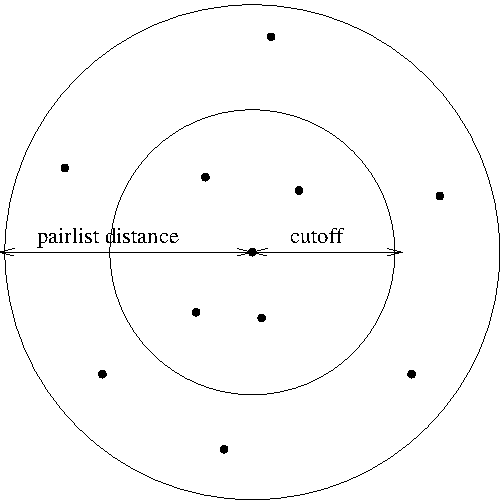
\includegraphics{figures/pairlistdist}}
  \caption[Example of cutoff and pairlist distance uses]
  {{\small Depiction of the difference between the cutoff distance and the
  pair list distance.  The pair list distance specifies a sphere that is
  slightly larger than that of the cutoff so that pairs are allowed to
  move in and out of the cutoff distance without causing energy conservation
  to be disturbed.}}
  \label{fig:pairlistdist}
\end{figure}

The {\tt pairlistdist} parameter is also used to determine the minimum patch size.
Unless the {\tt splitPatch} parameter is explicitly set to {\tt position}, hydrogen atoms will be placed on the same patch as the ``mother atom'' to which they are bonded.
These {\em hydrogen groups} are then distance tested against each other using only a cutoff increased by the the value of the {\tt hgroupCutoff} parameter.
The size of the patches is also increased by this amount.
\NAMD\ functions correctly even if a hydrogen atom and its mother atom are separated by more than half of {\tt hgroupCutoff} by breaking that group into its individual atoms for distance testing.
Margin violation warning messages are printed if an atom moves outside of a safe zone surrounding the patch to which it is assigned, indicating that {\tt pairlistdist} should be increased in order for forces to be calculated correctly and energy to be conserved.

\index{margin violations}
Margin violations mean that atoms that are in non-neighboring patches may
be closer than the cutoff distance apart.  This may sometimes happen in
constant pressure simulations when the cell shrinks (since the patch grid
remains the same size).  The workaround is to increase the margin
parameter so that the simulation starts with fewer, larger patches.
Restarting the simulation will also regenerate the patch grid.

In rare special circumstances atoms that are involved in bonded terms
(bonds, angles, dihedrals, or impropers) or nonbonded exclusions (especially
implicit exclusions due to bonds) will be placed on non-neighboring
patches because they are more than the cutoff distance apart.  This can
result in the simulation dying with a message of
``bad global exclusion count''.
\index{Atoms moving too fast}
\index{error message!Atoms moving too fast}
\index{Bad global exclusion count}
\index{error message!Bad global exclusion count}
If an ``atoms moving too fast; simulation has become unstable'',
``bad global exclusion count'', or similar error happens
on the first timestep then there is likely something very
wrong with the input coordinates, such as the atoms with uninitialized
coordinates or different atom orders in the PSF and PDB file.  Looking at
the system in VMD will often reveal an abnormal structure.
Be aware that the atom IDs in the ``Atoms moving too fast'' error
message are 1-based, while VMD's atom indices are 0-based.
If an ``atoms moving too fast; simulation has become unstable'',
``bad global exclusion count'', or similar error happens
later in the simulation then the dynamics have
probably become unstable, resulting in the system ``exploding'' apart.
Energies printed at every timestep should show an exponential increase.
This may be due to a timestep that is too long, or some other strange
feature.  Saving a trajectory of every step and working backwards in
can also sometimes reveal the origin of the instability.


\begin{itemize}

\item
\NAMDCONFWDEF{pairlistdist}
{distance between pairs for inclusion in pair lists (\AA)}
{positive decimal $\geq$ {\tt cutoff}}
{{\tt cutoff}}
{
A pair list is generated {\tt pairlistsPerCycle} times each cycle, 
containing pairs of atoms for which 
electrostatics and van der Waals interactions will be calculated.
This parameter is used when {\tt switching} is set to {\tt on} to
specify the allowable distance between atoms for inclusion in the
pair list.  
This parameter is equivalent to the X-PLOR parameter {\tt CUTNb}.
If no atom moves more than {\tt pairlistdist}$-${\tt cutoff} during
one cycle, then there will be no jump in electrostatic or van der
Waals energies when the next pair list is built.  Since such a jump
is unavoidable when truncation is used, this parameter may only
be specified when {\tt switching} is set to {\tt on}.  If this
parameter is not specified and {\tt switching} is set to {\tt on},
the value of {\tt cutoff} is used.  
A value of at least one greater than {\tt cutoff} is recommended.  
}

\item
\NAMDCONFWDEF{stepspercycle}{timesteps per cycle}{positive integer}{20}
{Number of timesteps in each cycle.  Each cycle represents the number 
of timesteps between the reassignment of atoms to patches, a procedure
referred to as \emph{atom migration}.
For more details on non-bonded force evaluation, see
Section \ref{section:electdesc}.}

\item
\NAMDCONFWDEF{splitPatch}
{how to assign atoms to patches}
{{\tt position} or {\tt hydrogen}}
{{\tt hydrogen}}
{
When set to {\tt hydrogen}, hydrogen atoms are kept on the same patch as their parents, allowing faster distance checking and rigid bonds.
}

\item
\NAMDCONFWDEF{hgroupCutoff (\AA)}
{used for group-based distance testing}
{positive decimal}
{2.5}
{
This should be set to twice the largest distance which will ever occur between a hydrogen atom and its mother.  Warnings will be printed if this is not the case.  This value is also added to the margin.
}

\item
\NAMDCONFWDEF{margin}
{extra length in patch dimension (\AA)}{positive decimal}{0.0}
{An internal tuning parameter used in determining the size of the cubes 
of space with which \NAMD\ uses to partition the system.  The value of 
this parameter will not change the physical results of the simulation.  
Unless you are very motivated to get the {\it very} best 
possible performance, just leave this value at the default.}

\item
\NAMDCONFWDEF{pairlistMinProcs}{min procs for pairlists}
{positive integer}{1}
{
Pairlists may consume a large amount of memory as atom counts, densities,
and cutoff distances increase.  Since this data is distributed across
processors it is normally only problematic for small processor counts.
Set pairlistMinProcs to the smallest number of processors on which
the simulation can fit into memory when pairlists are used.
}

\item
\NAMDCONFWDEF{pairlistsPerCycle}{regenerate x times per cycle}
{positive integer}{2}
{
Rather than only regenerating the pairlist at the beginning of a cycle,
regenerate multiple times in order to better balance the costs of
atom migration, pairlist generation, and larger pairlists.
}

\item
\NAMDCONFWDEF{outputPairlists}{how often to print warnings}
{non-negative integer}{0}
{
If an atom moves further than the pairlist tolerance during a simulation
(initially (pairlistdist - cutoff)/2 but refined during the run) any
pairlists covering that atom are invalidated and temporary pairlists
are used until the next full pairlist regeneration.  All interactions
are calculated correctly, but efficiency may be degraded.  Enabling
outputPairlists will summarize these pairlist violation warnings
periodically during the run.
}

\item
\NAMDCONFWDEF{pairlistShrink}{tol *= (1 - x) on regeneration}
{non-negative decimal}{0.01}
{
In order to maintain validity for the pairlist for an entire cycle,
the pairlist tolerance (the distance an atom can move without causing
the pairlist to be invalidated) is adjusted during the simulation.
Every time pairlists are regenerated the tolerance is reduced by
this fraction.
}

\item
\NAMDCONFWDEF{pairlistGrow}{tol *= (1 + x) on trigger}
{non-negative decimal}{0.01}
{
In order to maintain validity for the pairlist for an entire cycle,
the pairlist tolerance (the distance an atom can move without causing
the pairlist to be invalidated) is adjusted during the simulation.
Every time an atom exceeds a trigger criterion that is some fraction
of the tolerance distance, the tolerance is increased by this fraction.
}

\item
\NAMDCONFWDEF{pairlistTrigger}{trigger is atom beyond (1 - x) * tol}
{non-negative decimal}{0.3}
{
The goal of pairlist tolerance adjustment is to make pairlist invalidations
rare while keeping the tolerance as small as possible for best performance.
Rather than monitoring the (very rare) case where atoms actually move more
than the tolerance distance, we reduce the trigger tolerance by this
fraction.  The tolerance is increased whenever the trigger tolerance is
exceeded, as specified by pairlistGrow.
}

\end{itemize}

GPU-resident mode changes the default \texttt{margin} to 4\;{\AA}
to improve performance.
Since setting this parameter in the config file will override
this default, it is important for \texttt{margin} to remain \emph{unset}
without first running benchmarking experiments to find an optimal value.
Although \texttt{outputEnergies} will default to 100 steps,
this tends to be much too short for all but the largest
GPU-resident simulations.
It is recommended to set \texttt{outputEnergies}
to no less than 500 steps, maybe as high as 1000 or more.
To monitor performance, \texttt{outputTiming}
can be set to the same value as \texttt{outputEnergies}.
